% The full Promela model, with the LTL properties for the CWP, is in a public Github repository \cite{repo}. 
% The \emph{README.md} file in the repository summarizes its content and how to verify the model. 
% The model is divided into three files: the CWP object state, the CWP LTL properties, and the BPMN workflow. A script, \emph{short-verify.sh}, combines the three files to create the Promela model and then runs SPIN on all the properties.

\begin{comment}
\begin{figure*}[t]
  \begin{center}
    \begin{tabular}{c}
      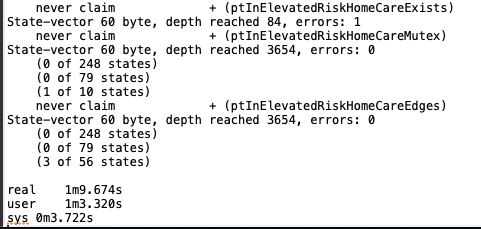
\includegraphics[scale=0.60]{../figs/proof-digest.png}
    \end{tabular}
  \end{center}
\caption{Some of the verification results from the SPIN model checker.}
\label{fig:proof}
\end{figure*}
The results for the state properties for \texttt{ptInElevatedRiskHomeCare} with the measured time verifying the entire model is shown in \figref{fig:proof}.
\end{comment}

\begin{comment}
As a reminder, the model and properties can be found at \cite{repo}.
Verification takes three to four minutes on an Intel Core i7 laptop with 16 Gb of RAM. It does not tax the system in any way.
All the existential properties (i.e., the properties ending with \emph{Exists}) resulted in an error. The error is the existential witness.
All other properties pass with no errors. The script's output includes not just the error report but the coverage summary of the processes and properties.
The first two entries pertain to the clinician and patient-caregiver processes. There should never be uncovered states in these processes.
Uncovered states means that there are unreachable behaviors in the model---not good. The third entry is the property being verified.
It is not unusual to have uncovered states here when there is no reported error since the error behavior is not found in the model---good.

To illustrate the value of model checking during design, it found many subtle errors during BPMN development.
Also in an early version of the CWP, SPIN found a trace through the workflow where the patient expires while in appropriate home care which is not allowed by the CWP. The error was in the CWP because the meaning of appropriate home care was not precise. It omitted information about trending severity that would indicate an elevated risk. The domain experts reviewed and approved changes to the transition conditions in the CWP, and SPIN then verified that the workflow preserved the property that patients only expire in elevated risk or in the hospital under those changed conditions. The very act of verifying the workflow against the CWP, even assuming the CWP is correct, yields important insights that are easily missed by manual inspection with domain experts.
\end{comment}


